% Created by tikzDevice version 0.10.1 on 2017-11-22 12:37:14
% !TEX encoding = UTF-8 Unicode
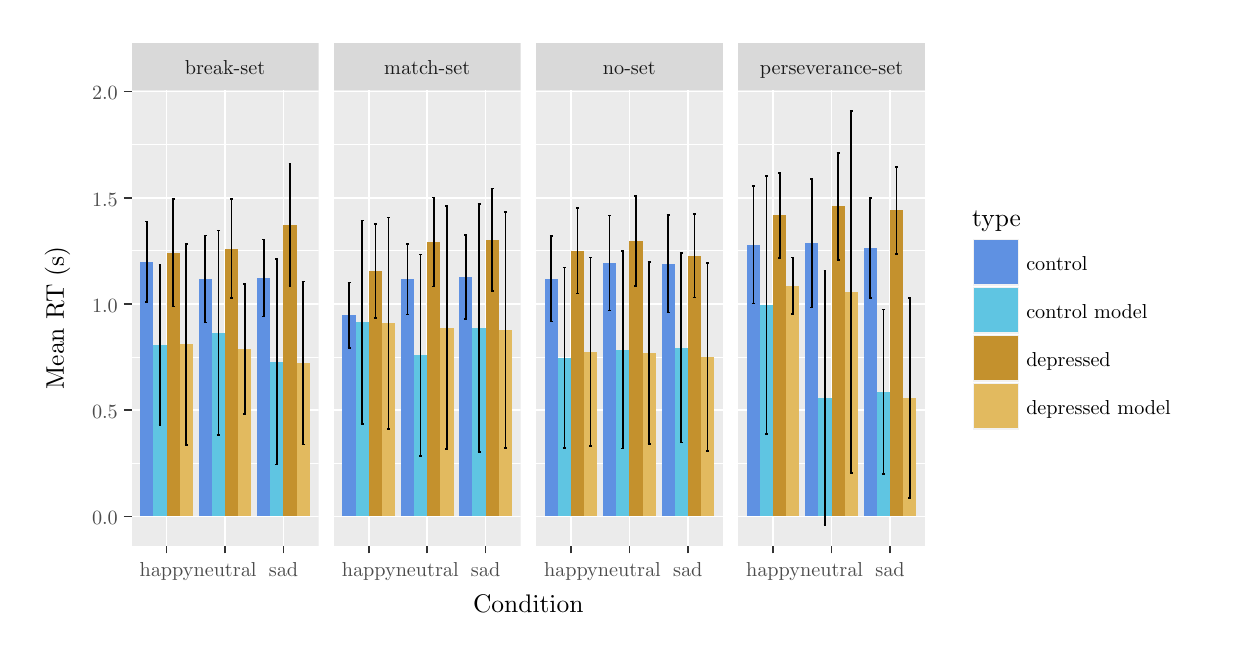
\begin{tikzpicture}[x=1pt,y=1pt]
\definecolor{fillColor}{RGB}{255,255,255}
\path[use as bounding box,fill=fillColor,fill opacity=0.00] (0,0) rectangle (433.62,216.81);
\begin{scope}
\path[clip] (  0.00,  0.00) rectangle (433.62,216.81);
\definecolor{drawColor}{RGB}{255,255,255}
\definecolor{fillColor}{RGB}{255,255,255}

\path[draw=drawColor,line width= 0.6pt,line join=round,line cap=round,fill=fillColor] (  0.00,  0.00) rectangle (433.62,216.81);
\end{scope}
\begin{scope}
\path[clip] ( 37.53, 29.59) rectangle (105.09,194.25);
\definecolor{fillColor}{gray}{0.92}

\path[fill=fillColor] ( 37.53, 29.59) rectangle (105.09,194.25);
\definecolor{drawColor}{RGB}{255,255,255}

\path[draw=drawColor,line width= 0.3pt,line join=round] ( 37.53, 59.37) --
	(105.09, 59.37);

\path[draw=drawColor,line width= 0.3pt,line join=round] ( 37.53, 97.75) --
	(105.09, 97.75);

\path[draw=drawColor,line width= 0.3pt,line join=round] ( 37.53,136.14) --
	(105.09,136.14);

\path[draw=drawColor,line width= 0.3pt,line join=round] ( 37.53,174.53) --
	(105.09,174.53);

\path[draw=drawColor,line width= 0.6pt,line join=round] ( 37.53, 40.18) --
	(105.09, 40.18);

\path[draw=drawColor,line width= 0.6pt,line join=round] ( 37.53, 78.56) --
	(105.09, 78.56);

\path[draw=drawColor,line width= 0.6pt,line join=round] ( 37.53,116.95) --
	(105.09,116.95);

\path[draw=drawColor,line width= 0.6pt,line join=round] ( 37.53,155.33) --
	(105.09,155.33);

\path[draw=drawColor,line width= 0.6pt,line join=round] ( 37.53,193.72) --
	(105.09,193.72);

\path[draw=drawColor,line width= 0.6pt,line join=round] ( 50.20, 29.59) --
	( 50.20,194.25);

\path[draw=drawColor,line width= 0.6pt,line join=round] ( 71.31, 29.59) --
	( 71.31,194.25);

\path[draw=drawColor,line width= 0.6pt,line join=round] ( 92.42, 29.59) --
	( 92.42,194.25);
\definecolor{fillColor}{RGB}{226,186,95}

\path[fill=fillColor] ( 54.95, 40.18) rectangle ( 59.70,102.38);
\definecolor{fillColor}{RGB}{196,145,45}

\path[fill=fillColor] ( 50.20, 40.18) rectangle ( 54.95,135.45);
\definecolor{fillColor}{RGB}{95,197,226}

\path[fill=fillColor] ( 45.45, 40.18) rectangle ( 50.20,102.13);
\definecolor{fillColor}{RGB}{95,145,226}

\path[fill=fillColor] ( 40.70, 40.18) rectangle ( 45.45,132.23);
\definecolor{fillColor}{RGB}{226,186,95}

\path[fill=fillColor] ( 76.06, 40.18) rectangle ( 80.81,100.66);
\definecolor{fillColor}{RGB}{196,145,45}

\path[fill=fillColor] ( 71.31, 40.18) rectangle ( 76.06,136.99);
\definecolor{fillColor}{RGB}{95,197,226}

\path[fill=fillColor] ( 66.56, 40.18) rectangle ( 71.31,106.64);
\definecolor{fillColor}{RGB}{95,145,226}

\path[fill=fillColor] ( 61.81, 40.18) rectangle ( 66.56,126.01);
\definecolor{fillColor}{RGB}{226,186,95}

\path[fill=fillColor] ( 97.17, 40.18) rectangle (101.92, 95.64);
\definecolor{fillColor}{RGB}{196,145,45}

\path[fill=fillColor] ( 92.42, 40.18) rectangle ( 97.17,145.66);
\definecolor{fillColor}{RGB}{95,197,226}

\path[fill=fillColor] ( 87.67, 40.18) rectangle ( 92.42, 96.08);
\definecolor{fillColor}{RGB}{95,145,226}

\path[fill=fillColor] ( 82.92, 40.18) rectangle ( 87.67,126.39);
\definecolor{drawColor}{RGB}{0,0,0}

\path[draw=drawColor,line width= 0.6pt,line join=round] ( 56.80,138.74) --
	( 57.85,138.74);

\path[draw=drawColor,line width= 0.6pt,line join=round] ( 57.32,138.74) --
	( 57.32, 66.02);

\path[draw=drawColor,line width= 0.6pt,line join=round] ( 56.80, 66.02) --
	( 57.85, 66.02);

\path[draw=drawColor,line width= 0.6pt,line join=round] ( 52.05,154.87) --
	( 53.10,154.87);

\path[draw=drawColor,line width= 0.6pt,line join=round] ( 52.57,154.87) --
	( 52.57,116.03);

\path[draw=drawColor,line width= 0.6pt,line join=round] ( 52.05,116.03) --
	( 53.10,116.03);

\path[draw=drawColor,line width= 0.6pt,line join=round] ( 47.30,131.11) --
	( 48.35,131.11);

\path[draw=drawColor,line width= 0.6pt,line join=round] ( 47.82,131.11) --
	( 47.82, 73.15);

\path[draw=drawColor,line width= 0.6pt,line join=round] ( 47.30, 73.15) --
	( 48.35, 73.15);

\path[draw=drawColor,line width= 0.6pt,line join=round] ( 42.55,146.74) --
	( 43.60,146.74);

\path[draw=drawColor,line width= 0.6pt,line join=round] ( 43.07,146.74) --
	( 43.07,117.72);

\path[draw=drawColor,line width= 0.6pt,line join=round] ( 42.55,117.72) --
	( 43.60,117.72);

\path[draw=drawColor,line width= 0.6pt,line join=round] ( 77.91,124.21) --
	( 78.96,124.21);

\path[draw=drawColor,line width= 0.6pt,line join=round] ( 78.44,124.21) --
	( 78.44, 77.12);

\path[draw=drawColor,line width= 0.6pt,line join=round] ( 77.91, 77.12) --
	( 78.96, 77.12);

\path[draw=drawColor,line width= 0.6pt,line join=round] ( 73.16,154.80) --
	( 74.21,154.80);

\path[draw=drawColor,line width= 0.6pt,line join=round] ( 73.69,154.80) --
	( 73.69,119.17);

\path[draw=drawColor,line width= 0.6pt,line join=round] ( 73.16,119.17) --
	( 74.21,119.17);

\path[draw=drawColor,line width= 0.6pt,line join=round] ( 68.41,143.55) --
	( 69.46,143.55);

\path[draw=drawColor,line width= 0.6pt,line join=round] ( 68.94,143.55) --
	( 68.94, 69.73);

\path[draw=drawColor,line width= 0.6pt,line join=round] ( 68.41, 69.73) --
	( 69.46, 69.73);

\path[draw=drawColor,line width= 0.6pt,line join=round] ( 63.66,141.75) --
	( 64.71,141.75);

\path[draw=drawColor,line width= 0.6pt,line join=round] ( 64.19,141.75) --
	( 64.19,110.27);

\path[draw=drawColor,line width= 0.6pt,line join=round] ( 63.66,110.27) --
	( 64.71,110.27);

\path[draw=drawColor,line width= 0.6pt,line join=round] ( 99.02,125.12) --
	(100.07,125.12);

\path[draw=drawColor,line width= 0.6pt,line join=round] ( 99.55,125.12) --
	( 99.55, 66.15);

\path[draw=drawColor,line width= 0.6pt,line join=round] ( 99.02, 66.15) --
	(100.07, 66.15);

\path[draw=drawColor,line width= 0.6pt,line join=round] ( 94.27,167.77) --
	( 95.32,167.77);

\path[draw=drawColor,line width= 0.6pt,line join=round] ( 94.80,167.77) --
	( 94.80,123.55);

\path[draw=drawColor,line width= 0.6pt,line join=round] ( 94.27,123.55) --
	( 95.32,123.55);

\path[draw=drawColor,line width= 0.6pt,line join=round] ( 89.52,133.22) --
	( 90.57,133.22);

\path[draw=drawColor,line width= 0.6pt,line join=round] ( 90.05,133.22) --
	( 90.05, 58.94);

\path[draw=drawColor,line width= 0.6pt,line join=round] ( 89.52, 58.94) --
	( 90.57, 58.94);

\path[draw=drawColor,line width= 0.6pt,line join=round] ( 84.77,140.29) --
	( 85.82,140.29);

\path[draw=drawColor,line width= 0.6pt,line join=round] ( 85.30,140.29) --
	( 85.30,112.50);

\path[draw=drawColor,line width= 0.6pt,line join=round] ( 84.77,112.50) --
	( 85.82,112.50);
\end{scope}
\begin{scope}
\path[clip] (110.59, 29.59) rectangle (178.14,194.25);
\definecolor{fillColor}{gray}{0.92}

\path[fill=fillColor] (110.59, 29.59) rectangle (178.14,194.25);
\definecolor{drawColor}{RGB}{255,255,255}

\path[draw=drawColor,line width= 0.3pt,line join=round] (110.59, 59.37) --
	(178.14, 59.37);

\path[draw=drawColor,line width= 0.3pt,line join=round] (110.59, 97.75) --
	(178.14, 97.75);

\path[draw=drawColor,line width= 0.3pt,line join=round] (110.59,136.14) --
	(178.14,136.14);

\path[draw=drawColor,line width= 0.3pt,line join=round] (110.59,174.53) --
	(178.14,174.53);

\path[draw=drawColor,line width= 0.6pt,line join=round] (110.59, 40.18) --
	(178.14, 40.18);

\path[draw=drawColor,line width= 0.6pt,line join=round] (110.59, 78.56) --
	(178.14, 78.56);

\path[draw=drawColor,line width= 0.6pt,line join=round] (110.59,116.95) --
	(178.14,116.95);

\path[draw=drawColor,line width= 0.6pt,line join=round] (110.59,155.33) --
	(178.14,155.33);

\path[draw=drawColor,line width= 0.6pt,line join=round] (110.59,193.72) --
	(178.14,193.72);

\path[draw=drawColor,line width= 0.6pt,line join=round] (123.25, 29.59) --
	(123.25,194.25);

\path[draw=drawColor,line width= 0.6pt,line join=round] (144.37, 29.59) --
	(144.37,194.25);

\path[draw=drawColor,line width= 0.6pt,line join=round] (165.48, 29.59) --
	(165.48,194.25);
\definecolor{fillColor}{RGB}{226,186,95}

\path[fill=fillColor] (128.00, 40.18) rectangle (132.75,110.04);
\definecolor{fillColor}{RGB}{196,145,45}

\path[fill=fillColor] (123.25, 40.18) rectangle (128.00,128.92);
\definecolor{fillColor}{RGB}{95,197,226}

\path[fill=fillColor] (118.50, 40.18) rectangle (123.25,110.39);
\definecolor{fillColor}{RGB}{95,145,226}

\path[fill=fillColor] (113.75, 40.18) rectangle (118.50,112.96);
\definecolor{fillColor}{RGB}{226,186,95}

\path[fill=fillColor] (149.12, 40.18) rectangle (153.87,108.46);
\definecolor{fillColor}{RGB}{196,145,45}

\path[fill=fillColor] (144.37, 40.18) rectangle (149.12,139.37);
\definecolor{fillColor}{RGB}{95,197,226}

\path[fill=fillColor] (139.62, 40.18) rectangle (144.37, 98.42);
\definecolor{fillColor}{RGB}{95,145,226}

\path[fill=fillColor] (134.87, 40.18) rectangle (139.62,125.93);
\definecolor{fillColor}{RGB}{226,186,95}

\path[fill=fillColor] (170.23, 40.18) rectangle (174.98,107.57);
\definecolor{fillColor}{RGB}{196,145,45}

\path[fill=fillColor] (165.48, 40.18) rectangle (170.23,140.13);
\definecolor{fillColor}{RGB}{95,197,226}

\path[fill=fillColor] (160.73, 40.18) rectangle (165.48,108.35);
\definecolor{fillColor}{RGB}{95,145,226}

\path[fill=fillColor] (155.98, 40.18) rectangle (160.73,126.70);
\definecolor{drawColor}{RGB}{0,0,0}

\path[draw=drawColor,line width= 0.6pt,line join=round] (129.85,148.23) --
	(130.91,148.23);

\path[draw=drawColor,line width= 0.6pt,line join=round] (130.38,148.23) --
	(130.38, 71.85);

\path[draw=drawColor,line width= 0.6pt,line join=round] (129.85, 71.85) --
	(130.91, 71.85);

\path[draw=drawColor,line width= 0.6pt,line join=round] (125.10,145.97) --
	(126.16,145.97);

\path[draw=drawColor,line width= 0.6pt,line join=round] (125.63,145.97) --
	(125.63,111.88);

\path[draw=drawColor,line width= 0.6pt,line join=round] (125.10,111.88) --
	(126.16,111.88);

\path[draw=drawColor,line width= 0.6pt,line join=round] (120.35,147.12) --
	(121.41,147.12);

\path[draw=drawColor,line width= 0.6pt,line join=round] (120.88,147.12) --
	(120.88, 73.66);

\path[draw=drawColor,line width= 0.6pt,line join=round] (120.35, 73.66) --
	(121.41, 73.66);

\path[draw=drawColor,line width= 0.6pt,line join=round] (115.60,124.78) --
	(116.66,124.78);

\path[draw=drawColor,line width= 0.6pt,line join=round] (116.13,124.78) --
	(116.13,101.13);

\path[draw=drawColor,line width= 0.6pt,line join=round] (115.60,101.13) --
	(116.66,101.13);

\path[draw=drawColor,line width= 0.6pt,line join=round] (150.96,152.31) --
	(152.02,152.31);

\path[draw=drawColor,line width= 0.6pt,line join=round] (151.49,152.31) --
	(151.49, 64.61);

\path[draw=drawColor,line width= 0.6pt,line join=round] (150.96, 64.61) --
	(152.02, 64.61);

\path[draw=drawColor,line width= 0.6pt,line join=round] (146.21,155.41) --
	(147.27,155.41);

\path[draw=drawColor,line width= 0.6pt,line join=round] (146.74,155.41) --
	(146.74,123.32);

\path[draw=drawColor,line width= 0.6pt,line join=round] (146.21,123.32) --
	(147.27,123.32);

\path[draw=drawColor,line width= 0.6pt,line join=round] (141.46,134.87) --
	(142.52,134.87);

\path[draw=drawColor,line width= 0.6pt,line join=round] (141.99,134.87) --
	(141.99, 61.96);

\path[draw=drawColor,line width= 0.6pt,line join=round] (141.46, 61.96) --
	(142.52, 61.96);

\path[draw=drawColor,line width= 0.6pt,line join=round] (136.71,138.75) --
	(137.77,138.75);

\path[draw=drawColor,line width= 0.6pt,line join=round] (137.24,138.75) --
	(137.24,113.11);

\path[draw=drawColor,line width= 0.6pt,line join=round] (136.71,113.11) --
	(137.77,113.11);

\path[draw=drawColor,line width= 0.6pt,line join=round] (172.07,150.09) --
	(173.13,150.09);

\path[draw=drawColor,line width= 0.6pt,line join=round] (172.60,150.09) --
	(172.60, 65.04);

\path[draw=drawColor,line width= 0.6pt,line join=round] (172.07, 65.04) --
	(173.13, 65.04);

\path[draw=drawColor,line width= 0.6pt,line join=round] (167.32,158.64) --
	(168.38,158.64);

\path[draw=drawColor,line width= 0.6pt,line join=round] (167.85,158.64) --
	(167.85,121.63);

\path[draw=drawColor,line width= 0.6pt,line join=round] (167.32,121.63) --
	(168.38,121.63);

\path[draw=drawColor,line width= 0.6pt,line join=round] (162.57,153.10) --
	(163.63,153.10);

\path[draw=drawColor,line width= 0.6pt,line join=round] (163.10,153.10) --
	(163.10, 63.59);

\path[draw=drawColor,line width= 0.6pt,line join=round] (162.57, 63.59) --
	(163.63, 63.59);

\path[draw=drawColor,line width= 0.6pt,line join=round] (157.82,141.98) --
	(158.88,141.98);

\path[draw=drawColor,line width= 0.6pt,line join=round] (158.35,141.98) --
	(158.35,111.42);

\path[draw=drawColor,line width= 0.6pt,line join=round] (157.82,111.42) --
	(158.88,111.42);
\end{scope}
\begin{scope}
\path[clip] (183.64, 29.59) rectangle (251.20,194.25);
\definecolor{fillColor}{gray}{0.92}

\path[fill=fillColor] (183.64, 29.59) rectangle (251.20,194.25);
\definecolor{drawColor}{RGB}{255,255,255}

\path[draw=drawColor,line width= 0.3pt,line join=round] (183.64, 59.37) --
	(251.20, 59.37);

\path[draw=drawColor,line width= 0.3pt,line join=round] (183.64, 97.75) --
	(251.20, 97.75);

\path[draw=drawColor,line width= 0.3pt,line join=round] (183.64,136.14) --
	(251.20,136.14);

\path[draw=drawColor,line width= 0.3pt,line join=round] (183.64,174.53) --
	(251.20,174.53);

\path[draw=drawColor,line width= 0.6pt,line join=round] (183.64, 40.18) --
	(251.20, 40.18);

\path[draw=drawColor,line width= 0.6pt,line join=round] (183.64, 78.56) --
	(251.20, 78.56);

\path[draw=drawColor,line width= 0.6pt,line join=round] (183.64,116.95) --
	(251.20,116.95);

\path[draw=drawColor,line width= 0.6pt,line join=round] (183.64,155.33) --
	(251.20,155.33);

\path[draw=drawColor,line width= 0.6pt,line join=round] (183.64,193.72) --
	(251.20,193.72);

\path[draw=drawColor,line width= 0.6pt,line join=round] (196.31, 29.59) --
	(196.31,194.25);

\path[draw=drawColor,line width= 0.6pt,line join=round] (217.42, 29.59) --
	(217.42,194.25);

\path[draw=drawColor,line width= 0.6pt,line join=round] (238.53, 29.59) --
	(238.53,194.25);
\definecolor{fillColor}{RGB}{226,186,95}

\path[fill=fillColor] (201.06, 40.18) rectangle (205.81, 99.69);
\definecolor{fillColor}{RGB}{196,145,45}

\path[fill=fillColor] (196.31, 40.18) rectangle (201.06,136.22);
\definecolor{fillColor}{RGB}{95,197,226}

\path[fill=fillColor] (191.56, 40.18) rectangle (196.31, 97.55);
\definecolor{fillColor}{RGB}{95,145,226}

\path[fill=fillColor] (186.81, 40.18) rectangle (191.56,126.08);
\definecolor{fillColor}{RGB}{226,186,95}

\path[fill=fillColor] (222.17, 40.18) rectangle (226.92, 99.23);
\definecolor{fillColor}{RGB}{196,145,45}

\path[fill=fillColor] (217.42, 40.18) rectangle (222.17,139.67);
\definecolor{fillColor}{RGB}{95,197,226}

\path[fill=fillColor] (212.67, 40.18) rectangle (217.42,100.44);
\definecolor{fillColor}{RGB}{95,145,226}

\path[fill=fillColor] (207.92, 40.18) rectangle (212.67,131.77);
\definecolor{fillColor}{RGB}{226,186,95}

\path[fill=fillColor] (243.28, 40.18) rectangle (248.03, 97.81);
\definecolor{fillColor}{RGB}{196,145,45}

\path[fill=fillColor] (238.53, 40.18) rectangle (243.28,134.45);
\definecolor{fillColor}{RGB}{95,197,226}

\path[fill=fillColor] (233.78, 40.18) rectangle (238.53,101.18);
\definecolor{fillColor}{RGB}{95,145,226}

\path[fill=fillColor] (229.03, 40.18) rectangle (233.78,131.54);
\definecolor{drawColor}{RGB}{0,0,0}

\path[draw=drawColor,line width= 0.6pt,line join=round] (202.91,133.81) --
	(203.96,133.81);

\path[draw=drawColor,line width= 0.6pt,line join=round] (203.43,133.81) --
	(203.43, 65.57);

\path[draw=drawColor,line width= 0.6pt,line join=round] (202.91, 65.57) --
	(203.96, 65.57);

\path[draw=drawColor,line width= 0.6pt,line join=round] (198.16,151.73) --
	(199.21,151.73);

\path[draw=drawColor,line width= 0.6pt,line join=round] (198.68,151.73) --
	(198.68,120.71);

\path[draw=drawColor,line width= 0.6pt,line join=round] (198.16,120.71) --
	(199.21,120.71);

\path[draw=drawColor,line width= 0.6pt,line join=round] (193.41,130.09) --
	(194.46,130.09);

\path[draw=drawColor,line width= 0.6pt,line join=round] (193.93,130.09) --
	(193.93, 65.01);

\path[draw=drawColor,line width= 0.6pt,line join=round] (193.41, 65.01) --
	(194.46, 65.01);

\path[draw=drawColor,line width= 0.6pt,line join=round] (188.66,141.52) --
	(189.71,141.52);

\path[draw=drawColor,line width= 0.6pt,line join=round] (189.18,141.52) --
	(189.18,110.65);

\path[draw=drawColor,line width= 0.6pt,line join=round] (188.66,110.65) --
	(189.71,110.65);

\path[draw=drawColor,line width= 0.6pt,line join=round] (224.02,132.03) --
	(225.07,132.03);

\path[draw=drawColor,line width= 0.6pt,line join=round] (224.55,132.03) --
	(224.55, 66.43);

\path[draw=drawColor,line width= 0.6pt,line join=round] (224.02, 66.43) --
	(225.07, 66.43);

\path[draw=drawColor,line width= 0.6pt,line join=round] (219.27,155.95) --
	(220.32,155.95);

\path[draw=drawColor,line width= 0.6pt,line join=round] (219.80,155.95) --
	(219.80,123.40);

\path[draw=drawColor,line width= 0.6pt,line join=round] (219.27,123.40) --
	(220.32,123.40);

\path[draw=drawColor,line width= 0.6pt,line join=round] (214.52,136.11) --
	(215.57,136.11);

\path[draw=drawColor,line width= 0.6pt,line join=round] (215.05,136.11) --
	(215.05, 64.77);

\path[draw=drawColor,line width= 0.6pt,line join=round] (214.52, 64.77) --
	(215.57, 64.77);

\path[draw=drawColor,line width= 0.6pt,line join=round] (209.77,148.89) --
	(210.82,148.89);

\path[draw=drawColor,line width= 0.6pt,line join=round] (210.30,148.89) --
	(210.30,114.65);

\path[draw=drawColor,line width= 0.6pt,line join=round] (209.77,114.65) --
	(210.82,114.65);

\path[draw=drawColor,line width= 0.6pt,line join=round] (245.13,131.68) --
	(246.18,131.68);

\path[draw=drawColor,line width= 0.6pt,line join=round] (245.66,131.68) --
	(245.66, 63.95);

\path[draw=drawColor,line width= 0.6pt,line join=round] (245.13, 63.95) --
	(246.18, 63.95);

\path[draw=drawColor,line width= 0.6pt,line join=round] (240.38,149.58) --
	(241.43,149.58);

\path[draw=drawColor,line width= 0.6pt,line join=round] (240.91,149.58) --
	(240.91,119.33);

\path[draw=drawColor,line width= 0.6pt,line join=round] (240.38,119.33) --
	(241.43,119.33);

\path[draw=drawColor,line width= 0.6pt,line join=round] (235.63,135.43) --
	(236.68,135.43);

\path[draw=drawColor,line width= 0.6pt,line join=round] (236.16,135.43) --
	(236.16, 66.93);

\path[draw=drawColor,line width= 0.6pt,line join=round] (235.63, 66.93) --
	(236.68, 66.93);

\path[draw=drawColor,line width= 0.6pt,line join=round] (230.88,149.19) --
	(231.93,149.19);

\path[draw=drawColor,line width= 0.6pt,line join=round] (231.41,149.19) --
	(231.41,113.88);

\path[draw=drawColor,line width= 0.6pt,line join=round] (230.88,113.88) --
	(231.93,113.88);
\end{scope}
\begin{scope}
\path[clip] (256.70, 29.59) rectangle (324.25,194.25);
\definecolor{fillColor}{gray}{0.92}

\path[fill=fillColor] (256.70, 29.59) rectangle (324.25,194.25);
\definecolor{drawColor}{RGB}{255,255,255}

\path[draw=drawColor,line width= 0.3pt,line join=round] (256.70, 59.37) --
	(324.25, 59.37);

\path[draw=drawColor,line width= 0.3pt,line join=round] (256.70, 97.75) --
	(324.25, 97.75);

\path[draw=drawColor,line width= 0.3pt,line join=round] (256.70,136.14) --
	(324.25,136.14);

\path[draw=drawColor,line width= 0.3pt,line join=round] (256.70,174.53) --
	(324.25,174.53);

\path[draw=drawColor,line width= 0.6pt,line join=round] (256.70, 40.18) --
	(324.25, 40.18);

\path[draw=drawColor,line width= 0.6pt,line join=round] (256.70, 78.56) --
	(324.25, 78.56);

\path[draw=drawColor,line width= 0.6pt,line join=round] (256.70,116.95) --
	(324.25,116.95);

\path[draw=drawColor,line width= 0.6pt,line join=round] (256.70,155.33) --
	(324.25,155.33);

\path[draw=drawColor,line width= 0.6pt,line join=round] (256.70,193.72) --
	(324.25,193.72);

\path[draw=drawColor,line width= 0.6pt,line join=round] (269.36, 29.59) --
	(269.36,194.25);

\path[draw=drawColor,line width= 0.6pt,line join=round] (290.48, 29.59) --
	(290.48,194.25);

\path[draw=drawColor,line width= 0.6pt,line join=round] (311.59, 29.59) --
	(311.59,194.25);
\definecolor{fillColor}{RGB}{226,186,95}

\path[fill=fillColor] (274.11, 40.18) rectangle (278.86,123.51);
\definecolor{fillColor}{RGB}{196,145,45}

\path[fill=fillColor] (269.36, 40.18) rectangle (274.11,148.96);
\definecolor{fillColor}{RGB}{95,197,226}

\path[fill=fillColor] (264.61, 40.18) rectangle (269.36,116.65);
\definecolor{fillColor}{RGB}{95,145,226}

\path[fill=fillColor] (259.86, 40.18) rectangle (264.61,138.29);
\definecolor{fillColor}{RGB}{226,186,95}

\path[fill=fillColor] (295.23, 40.18) rectangle (299.98,121.36);
\definecolor{fillColor}{RGB}{196,145,45}

\path[fill=fillColor] (290.48, 40.18) rectangle (295.23,152.26);
\definecolor{fillColor}{RGB}{95,197,226}

\path[fill=fillColor] (285.73, 40.18) rectangle (290.48, 83.06);
\definecolor{fillColor}{RGB}{95,145,226}

\path[fill=fillColor] (280.98, 40.18) rectangle (285.73,138.91);
\definecolor{fillColor}{RGB}{226,186,95}

\path[fill=fillColor] (316.34, 40.18) rectangle (321.09, 82.92);
\definecolor{fillColor}{RGB}{196,145,45}

\path[fill=fillColor] (311.59, 40.18) rectangle (316.34,150.81);
\definecolor{fillColor}{RGB}{95,197,226}

\path[fill=fillColor] (306.84, 40.18) rectangle (311.59, 85.21);
\definecolor{fillColor}{RGB}{95,145,226}

\path[fill=fillColor] (302.09, 40.18) rectangle (306.84,137.14);
\definecolor{drawColor}{RGB}{0,0,0}

\path[draw=drawColor,line width= 0.6pt,line join=round] (275.96,133.79) --
	(277.02,133.79);

\path[draw=drawColor,line width= 0.6pt,line join=round] (276.49,133.79) --
	(276.49,113.23);

\path[draw=drawColor,line width= 0.6pt,line join=round] (275.96,113.23) --
	(277.02,113.23);

\path[draw=drawColor,line width= 0.6pt,line join=round] (271.21,164.39) --
	(272.27,164.39);

\path[draw=drawColor,line width= 0.6pt,line join=round] (271.74,164.39) --
	(271.74,133.53);

\path[draw=drawColor,line width= 0.6pt,line join=round] (271.21,133.53) --
	(272.27,133.53);

\path[draw=drawColor,line width= 0.6pt,line join=round] (266.46,163.19) --
	(267.52,163.19);

\path[draw=drawColor,line width= 0.6pt,line join=round] (266.99,163.19) --
	(266.99, 70.10);

\path[draw=drawColor,line width= 0.6pt,line join=round] (266.46, 70.10) --
	(267.52, 70.10);

\path[draw=drawColor,line width= 0.6pt,line join=round] (261.71,159.48) --
	(262.77,159.48);

\path[draw=drawColor,line width= 0.6pt,line join=round] (262.24,159.48) --
	(262.24,117.10);

\path[draw=drawColor,line width= 0.6pt,line join=round] (261.71,117.10) --
	(262.77,117.10);

\path[draw=drawColor,line width= 0.6pt,line join=round] (297.07,186.76) --
	(298.13,186.76);

\path[draw=drawColor,line width= 0.6pt,line join=round] (297.60,186.76) --
	(297.60, 55.95);

\path[draw=drawColor,line width= 0.6pt,line join=round] (297.07, 55.95) --
	(298.13, 55.95);

\path[draw=drawColor,line width= 0.6pt,line join=round] (292.32,171.61) --
	(293.38,171.61);

\path[draw=drawColor,line width= 0.6pt,line join=round] (292.85,171.61) --
	(292.85,132.92);

\path[draw=drawColor,line width= 0.6pt,line join=round] (292.32,132.92) --
	(293.38,132.92);

\path[draw=drawColor,line width= 0.6pt,line join=round] (287.57,129.06) --
	(288.63,129.06);

\path[draw=drawColor,line width= 0.6pt,line join=round] (288.10,129.06) --
	(288.10, 37.07);

\path[draw=drawColor,line width= 0.6pt,line join=round] (287.57, 37.07) --
	(288.63, 37.07);

\path[draw=drawColor,line width= 0.6pt,line join=round] (282.82,162.17) --
	(283.88,162.17);

\path[draw=drawColor,line width= 0.6pt,line join=round] (283.35,162.17) --
	(283.35,115.64);

\path[draw=drawColor,line width= 0.6pt,line join=round] (282.82,115.64) --
	(283.88,115.64);

\path[draw=drawColor,line width= 0.6pt,line join=round] (318.18,119.07) --
	(319.24,119.07);

\path[draw=drawColor,line width= 0.6pt,line join=round] (318.71,119.07) --
	(318.71, 46.76);

\path[draw=drawColor,line width= 0.6pt,line join=round] (318.18, 46.76) --
	(319.24, 46.76);

\path[draw=drawColor,line width= 0.6pt,line join=round] (313.43,166.54) --
	(314.49,166.54);

\path[draw=drawColor,line width= 0.6pt,line join=round] (313.96,166.54) --
	(313.96,135.07);

\path[draw=drawColor,line width= 0.6pt,line join=round] (313.43,135.07) --
	(314.49,135.07);

\path[draw=drawColor,line width= 0.6pt,line join=round] (308.68,114.96) --
	(309.74,114.96);

\path[draw=drawColor,line width= 0.6pt,line join=round] (309.21,114.96) --
	(309.21, 55.45);

\path[draw=drawColor,line width= 0.6pt,line join=round] (308.68, 55.45) --
	(309.74, 55.45);

\path[draw=drawColor,line width= 0.6pt,line join=round] (303.93,155.18) --
	(304.99,155.18);

\path[draw=drawColor,line width= 0.6pt,line join=round] (304.46,155.18) --
	(304.46,119.10);

\path[draw=drawColor,line width= 0.6pt,line join=round] (303.93,119.10) --
	(304.99,119.10);
\end{scope}
\begin{scope}
\path[clip] ( 37.53,194.25) rectangle (105.09,211.31);
\definecolor{fillColor}{gray}{0.85}

\path[fill=fillColor] ( 37.53,194.25) rectangle (105.09,211.31);
\definecolor{drawColor}{gray}{0.10}

\node[text=drawColor,anchor=base,inner sep=0pt, outer sep=0pt, scale=  0.73] at ( 71.31,199.75) {break-set};
\end{scope}
\begin{scope}
\path[clip] (110.59,194.25) rectangle (178.14,211.31);
\definecolor{fillColor}{gray}{0.85}

\path[fill=fillColor] (110.59,194.25) rectangle (178.14,211.31);
\definecolor{drawColor}{gray}{0.10}

\node[text=drawColor,anchor=base,inner sep=0pt, outer sep=0pt, scale=  0.73] at (144.37,199.75) {match-set};
\end{scope}
\begin{scope}
\path[clip] (183.64,194.25) rectangle (251.20,211.31);
\definecolor{fillColor}{gray}{0.85}

\path[fill=fillColor] (183.64,194.25) rectangle (251.20,211.31);
\definecolor{drawColor}{gray}{0.10}

\node[text=drawColor,anchor=base,inner sep=0pt, outer sep=0pt, scale=  0.73] at (217.42,199.75) {no-set};
\end{scope}
\begin{scope}
\path[clip] (256.70,194.25) rectangle (324.25,211.31);
\definecolor{fillColor}{gray}{0.85}

\path[fill=fillColor] (256.70,194.25) rectangle (324.25,211.31);
\definecolor{drawColor}{gray}{0.10}

\node[text=drawColor,anchor=base,inner sep=0pt, outer sep=0pt, scale=  0.73] at (290.48,199.75) {perseverance-set};
\end{scope}
\begin{scope}
\path[clip] (  0.00,  0.00) rectangle (433.62,216.81);
\definecolor{drawColor}{gray}{0.20}

\path[draw=drawColor,line width= 0.6pt,line join=round] ( 50.20, 26.84) --
	( 50.20, 29.59);

\path[draw=drawColor,line width= 0.6pt,line join=round] ( 71.31, 26.84) --
	( 71.31, 29.59);

\path[draw=drawColor,line width= 0.6pt,line join=round] ( 92.42, 26.84) --
	( 92.42, 29.59);
\end{scope}
\begin{scope}
\path[clip] (  0.00,  0.00) rectangle (433.62,216.81);
\definecolor{drawColor}{gray}{0.30}

\node[text=drawColor,anchor=base,inner sep=0pt, outer sep=0pt, scale=  0.73] at ( 50.20, 18.58) {happy};

\node[text=drawColor,anchor=base,inner sep=0pt, outer sep=0pt, scale=  0.73] at ( 71.31, 18.58) {neutral};

\node[text=drawColor,anchor=base,inner sep=0pt, outer sep=0pt, scale=  0.73] at ( 92.42, 18.58) {sad};
\end{scope}
\begin{scope}
\path[clip] (  0.00,  0.00) rectangle (433.62,216.81);
\definecolor{drawColor}{gray}{0.20}

\path[draw=drawColor,line width= 0.6pt,line join=round] (123.25, 26.84) --
	(123.25, 29.59);

\path[draw=drawColor,line width= 0.6pt,line join=round] (144.37, 26.84) --
	(144.37, 29.59);

\path[draw=drawColor,line width= 0.6pt,line join=round] (165.48, 26.84) --
	(165.48, 29.59);
\end{scope}
\begin{scope}
\path[clip] (  0.00,  0.00) rectangle (433.62,216.81);
\definecolor{drawColor}{gray}{0.30}

\node[text=drawColor,anchor=base,inner sep=0pt, outer sep=0pt, scale=  0.73] at (123.25, 18.58) {happy};

\node[text=drawColor,anchor=base,inner sep=0pt, outer sep=0pt, scale=  0.73] at (144.37, 18.58) {neutral};

\node[text=drawColor,anchor=base,inner sep=0pt, outer sep=0pt, scale=  0.73] at (165.48, 18.58) {sad};
\end{scope}
\begin{scope}
\path[clip] (  0.00,  0.00) rectangle (433.62,216.81);
\definecolor{drawColor}{gray}{0.20}

\path[draw=drawColor,line width= 0.6pt,line join=round] (196.31, 26.84) --
	(196.31, 29.59);

\path[draw=drawColor,line width= 0.6pt,line join=round] (217.42, 26.84) --
	(217.42, 29.59);

\path[draw=drawColor,line width= 0.6pt,line join=round] (238.53, 26.84) --
	(238.53, 29.59);
\end{scope}
\begin{scope}
\path[clip] (  0.00,  0.00) rectangle (433.62,216.81);
\definecolor{drawColor}{gray}{0.30}

\node[text=drawColor,anchor=base,inner sep=0pt, outer sep=0pt, scale=  0.73] at (196.31, 18.58) {happy};

\node[text=drawColor,anchor=base,inner sep=0pt, outer sep=0pt, scale=  0.73] at (217.42, 18.58) {neutral};

\node[text=drawColor,anchor=base,inner sep=0pt, outer sep=0pt, scale=  0.73] at (238.53, 18.58) {sad};
\end{scope}
\begin{scope}
\path[clip] (  0.00,  0.00) rectangle (433.62,216.81);
\definecolor{drawColor}{gray}{0.20}

\path[draw=drawColor,line width= 0.6pt,line join=round] (269.36, 26.84) --
	(269.36, 29.59);

\path[draw=drawColor,line width= 0.6pt,line join=round] (290.48, 26.84) --
	(290.48, 29.59);

\path[draw=drawColor,line width= 0.6pt,line join=round] (311.59, 26.84) --
	(311.59, 29.59);
\end{scope}
\begin{scope}
\path[clip] (  0.00,  0.00) rectangle (433.62,216.81);
\definecolor{drawColor}{gray}{0.30}

\node[text=drawColor,anchor=base,inner sep=0pt, outer sep=0pt, scale=  0.73] at (269.36, 18.58) {happy};

\node[text=drawColor,anchor=base,inner sep=0pt, outer sep=0pt, scale=  0.73] at (290.48, 18.58) {neutral};

\node[text=drawColor,anchor=base,inner sep=0pt, outer sep=0pt, scale=  0.73] at (311.59, 18.58) {sad};
\end{scope}
\begin{scope}
\path[clip] (  0.00,  0.00) rectangle (433.62,216.81);
\definecolor{drawColor}{gray}{0.30}

\node[text=drawColor,anchor=base east,inner sep=0pt, outer sep=0pt, scale=  0.73] at ( 32.58, 37.15) {0.0};

\node[text=drawColor,anchor=base east,inner sep=0pt, outer sep=0pt, scale=  0.73] at ( 32.58, 75.53) {0.5};

\node[text=drawColor,anchor=base east,inner sep=0pt, outer sep=0pt, scale=  0.73] at ( 32.58,113.92) {1.0};

\node[text=drawColor,anchor=base east,inner sep=0pt, outer sep=0pt, scale=  0.73] at ( 32.58,152.30) {1.5};

\node[text=drawColor,anchor=base east,inner sep=0pt, outer sep=0pt, scale=  0.73] at ( 32.58,190.69) {2.0};
\end{scope}
\begin{scope}
\path[clip] (  0.00,  0.00) rectangle (433.62,216.81);
\definecolor{drawColor}{gray}{0.20}

\path[draw=drawColor,line width= 0.6pt,line join=round] ( 34.78, 40.18) --
	( 37.53, 40.18);

\path[draw=drawColor,line width= 0.6pt,line join=round] ( 34.78, 78.56) --
	( 37.53, 78.56);

\path[draw=drawColor,line width= 0.6pt,line join=round] ( 34.78,116.95) --
	( 37.53,116.95);

\path[draw=drawColor,line width= 0.6pt,line join=round] ( 34.78,155.33) --
	( 37.53,155.33);

\path[draw=drawColor,line width= 0.6pt,line join=round] ( 34.78,193.72) --
	( 37.53,193.72);
\end{scope}
\begin{scope}
\path[clip] (  0.00,  0.00) rectangle (433.62,216.81);
\definecolor{drawColor}{RGB}{0,0,0}

\node[text=drawColor,anchor=base,inner sep=0pt, outer sep=0pt, scale=  0.92] at (180.89,  5.50) {Condition};
\end{scope}
\begin{scope}
\path[clip] (  0.00,  0.00) rectangle (433.62,216.81);
\definecolor{drawColor}{RGB}{0,0,0}

\node[text=drawColor,rotate= 90.00,anchor=base,inner sep=0pt, outer sep=0pt, scale=  0.92] at ( 13.08,111.92) {Mean RT (s)};
\end{scope}
\begin{scope}
\path[clip] (  0.00,  0.00) rectangle (433.62,216.81);
\definecolor{fillColor}{RGB}{255,255,255}

\path[fill=fillColor] (335.63, 65.58) rectangle (428.12,158.25);
\end{scope}
\begin{scope}
\path[clip] (  0.00,  0.00) rectangle (433.62,216.81);
\definecolor{drawColor}{RGB}{0,0,0}

\node[text=drawColor,anchor=base west,inner sep=0pt, outer sep=0pt, scale=  0.92] at (341.32,144.99) {type};
\end{scope}
\begin{scope}
\path[clip] (  0.00,  0.00) rectangle (433.62,216.81);
\definecolor{drawColor}{RGB}{255,255,255}
\definecolor{fillColor}{gray}{0.95}

\path[draw=drawColor,line width= 0.6pt,line join=round,line cap=round,fill=fillColor] (341.32,123.31) rectangle (358.67,140.65);
\end{scope}
\begin{scope}
\path[clip] (  0.00,  0.00) rectangle (433.62,216.81);
\definecolor{fillColor}{RGB}{95,145,226}

\path[fill=fillColor] (342.04,124.02) rectangle (357.96,139.94);
\end{scope}
\begin{scope}
\path[clip] (  0.00,  0.00) rectangle (433.62,216.81);
\definecolor{drawColor}{RGB}{255,255,255}
\definecolor{fillColor}{gray}{0.95}

\path[draw=drawColor,line width= 0.6pt,line join=round,line cap=round,fill=fillColor] (341.32,105.96) rectangle (358.67,123.31);
\end{scope}
\begin{scope}
\path[clip] (  0.00,  0.00) rectangle (433.62,216.81);
\definecolor{fillColor}{RGB}{95,197,226}

\path[fill=fillColor] (342.04,106.67) rectangle (357.96,122.60);
\end{scope}
\begin{scope}
\path[clip] (  0.00,  0.00) rectangle (433.62,216.81);
\definecolor{drawColor}{RGB}{255,255,255}
\definecolor{fillColor}{gray}{0.95}

\path[draw=drawColor,line width= 0.6pt,line join=round,line cap=round,fill=fillColor] (341.32, 88.62) rectangle (358.67,105.96);
\end{scope}
\begin{scope}
\path[clip] (  0.00,  0.00) rectangle (433.62,216.81);
\definecolor{fillColor}{RGB}{196,145,45}

\path[fill=fillColor] (342.04, 89.33) rectangle (357.96,105.25);
\end{scope}
\begin{scope}
\path[clip] (  0.00,  0.00) rectangle (433.62,216.81);
\definecolor{drawColor}{RGB}{255,255,255}
\definecolor{fillColor}{gray}{0.95}

\path[draw=drawColor,line width= 0.6pt,line join=round,line cap=round,fill=fillColor] (341.32, 71.27) rectangle (358.67, 88.62);
\end{scope}
\begin{scope}
\path[clip] (  0.00,  0.00) rectangle (433.62,216.81);
\definecolor{fillColor}{RGB}{226,186,95}

\path[fill=fillColor] (342.04, 71.98) rectangle (357.96, 87.91);
\end{scope}
\begin{scope}
\path[clip] (  0.00,  0.00) rectangle (433.62,216.81);
\definecolor{drawColor}{RGB}{0,0,0}

\node[text=drawColor,anchor=base west,inner sep=0pt, outer sep=0pt, scale=  0.73] at (360.84,128.95) {control};
\end{scope}
\begin{scope}
\path[clip] (  0.00,  0.00) rectangle (433.62,216.81);
\definecolor{drawColor}{RGB}{0,0,0}

\node[text=drawColor,anchor=base west,inner sep=0pt, outer sep=0pt, scale=  0.73] at (360.84,111.60) {control model};
\end{scope}
\begin{scope}
\path[clip] (  0.00,  0.00) rectangle (433.62,216.81);
\definecolor{drawColor}{RGB}{0,0,0}

\node[text=drawColor,anchor=base west,inner sep=0pt, outer sep=0pt, scale=  0.73] at (360.84, 94.26) {depressed};
\end{scope}
\begin{scope}
\path[clip] (  0.00,  0.00) rectangle (433.62,216.81);
\definecolor{drawColor}{RGB}{0,0,0}

\node[text=drawColor,anchor=base west,inner sep=0pt, outer sep=0pt, scale=  0.73] at (360.84, 76.91) {depressed model};
\end{scope}
\end{tikzpicture}
